\section{Rotation speed dependence of layer thicknesses}
\label{sec:rot}

In this section, we investigate the rotation speed dependence of layer thickness.


As depicted in Figure \ref{fig:VglMethRotThick}, the thickness declines for higher rotational speed. This is also what is expected from
the Schubert equation introduced in section \ref{sec:Schubert}. In the following the data is fitted using the Schubert equation.

\begin{figure}[ht]
    \centering
    \begin{subfigure}[b]{0.49\textwidth}
        \centering
        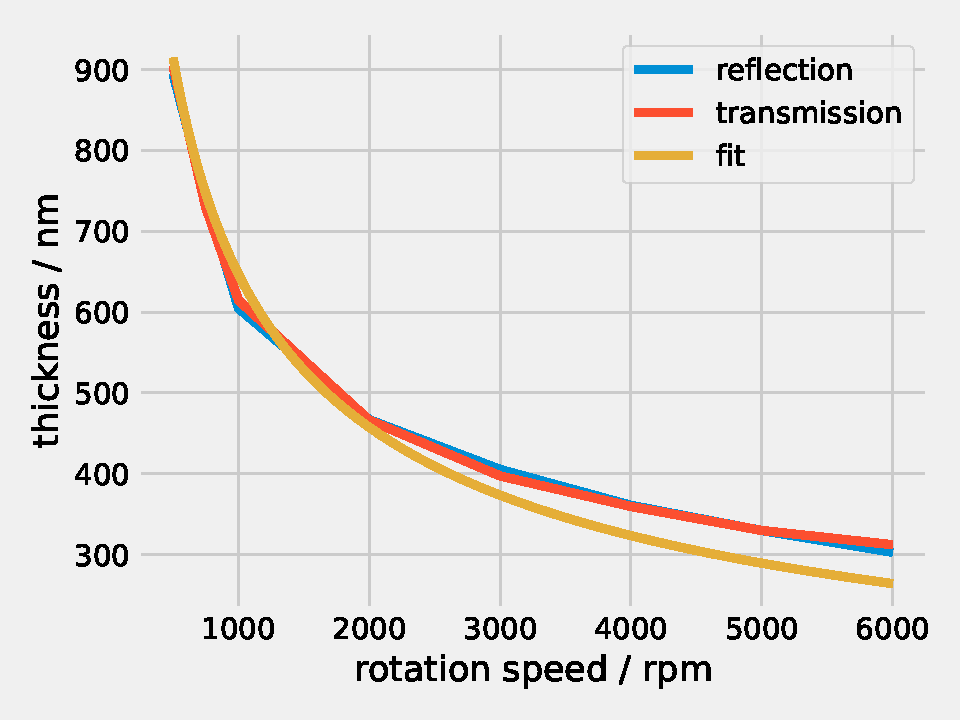
\includegraphics[width = \textwidth]{Programmien/RotFit500to6000.pdf}
        \caption{Thickness of the thin films in dependence of rotation speed}
        %\label{fig:y equals x}
    \end{subfigure}  
    \begin{subfigure}[b]{0.49\textwidth}
        \centering
        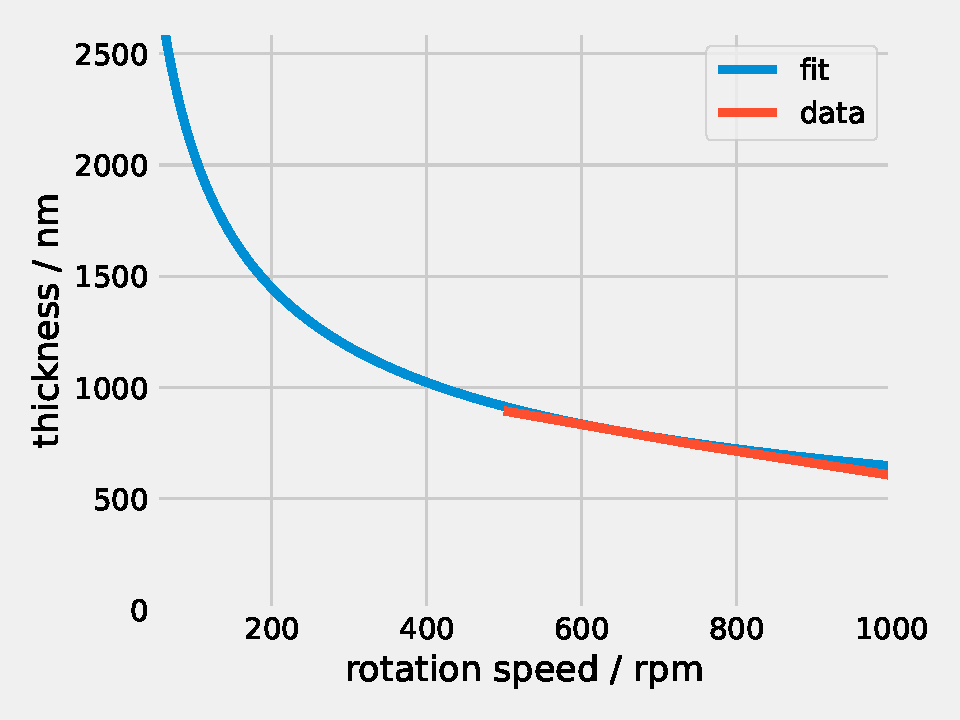
\includegraphics[width = \textwidth]{Programmien/RotFit0to1000.pdf}
        \caption{Thickness of the films extrapolated towards \SI{0}{rpm}}
        %\label{fig:y equals x}
    \end{subfigure}  

    \begin{subfigure}[b]{0.5\textwidth}
        \centering
        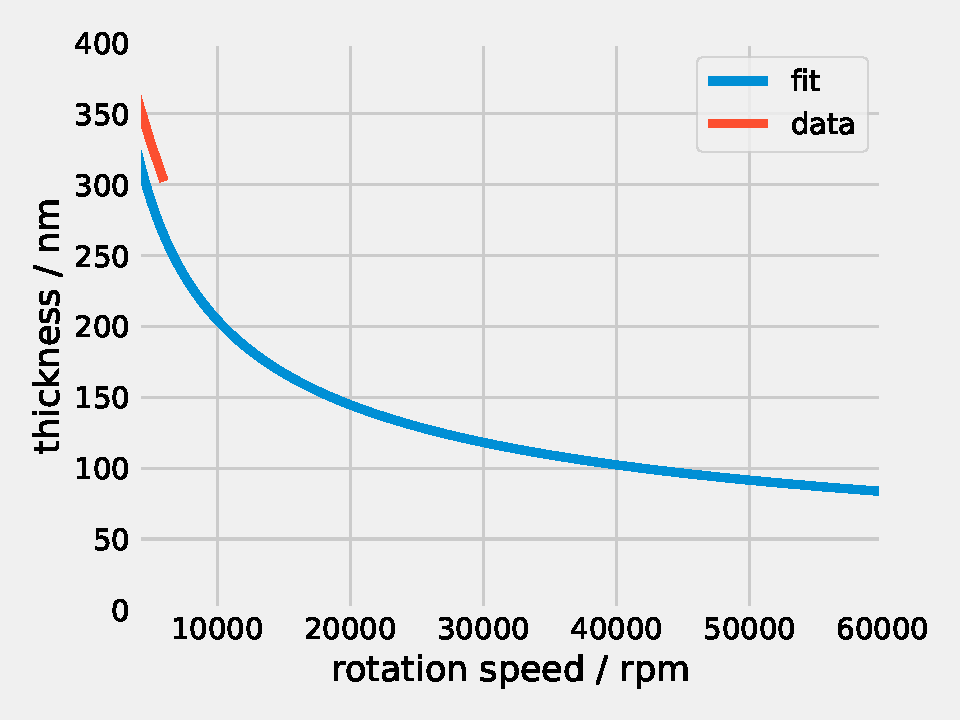
\includegraphics[width = \textwidth]{Programmien/RotFit5000to10000.pdf}
        \caption{Thickness of the films extrapolated towards higher rotational speed}
        %\label{fig:y equals x}
    \end{subfigure}  

    \caption{The film thickness in dependence of the rotational speed. The data is fitted in (a) with the Schubert equation and afterwards further values for the thickness $d$ are extrapolated in (b) and (c).}
    %\label{fig:SpecRefTrans}
\end{figure}


% The fit using the Schubert equation shows some minor discrepancies especially for higher rotation speeds. Those are caused among others by the unequal spacing between the data points.
% As a result the fit is better adjusted to the areas with higher "data density". When extrapolation the data using the Schubert equation, we observe a strong increase in thickness for lower rotational speed.
% In the limit for rotation speed against 0 rpm we observe diverging/ very high film thickness. This case is equivalent to normal drying of the film. With this production method, very inhomogeneous films are to be expected, since aggregates can form in the solution, drying is not homogeneous, and dewetting effects can cause spatial differences in the substrate.
% This is also in accordance with the observations about heterogeneity made in section \ref{sec:VglMeth}. For higher rotational speed the thick of the film declines with to a limes of \SI{0}{nm}. This is also to be expected since for infinly fast spinning, the
% rotational force get infinitely big. Therefore the drying solution on the substrate gets infinitely thin and therefore the dried film afterwards too.

The fit using the Schubert equation shows some minor discrepancies, especially for higher rotation speeds. Those are caused, among others, by the unequal spacing between the data points. As a result, the fit is better adjusted to the areas with higher "data density". When extrapolating the data using the Schubert equation, we observe a strong increase in film thickness for lower rotational speeds. In the limit for rotation speed against \SI{0}{rpm}, we observe diverging/ very high film thickness. This case is equivalent to normal drying of the film. With this production method, very heterogeneous films are to be expected, as aggregates can form in the solution, drying is not uniform, and dewetting effects can cause spatial differences on the substrate. This is also in accordance with the observations about heterogeneity made in section \ref{sec:VglMeth}. For higher rotational speeds, the thickness of the film declines to a limit of \SI{0}{nm}. This is also to be expected, as for infinitely fast spinning, the rotational force gets infinitely big. Therefore, the drying solution on the substrate gets infinitely thin, and the dried film will also be infinitely thin.
